\section{Auswertung}
\label{sec:Auswertung}
\subsection{Bestimmung der mittleren Reichweite}
Da der MCA nur Channel, keine konkreten Energien ausgibt, müssen diese über Dreisatz in Energien umgerechnet werden, wobei Channel 280 $\SI{4}{\mega \electronvolt}$ entspricht.
Aus dem in Abb.\ref{fig:Energie} mittels \eqref{eqn:gerade} gefitteten Ausgleich der ersten Messung erhält man die Parameter: $a_1 = \SI{-2.11 \pm 0.06}{\mega\eV}$, $b_1=\SI{4.06 \pm 0.03}{\mega\eV}$. Entsprechend liefert die zweite Messung $a_2 = \SI{-2.67 \pm 0.09}{\mega\eV}$, $b_2 = \SI{4.06 \pm 0.03}{\mega eV}$. Der Abstand der Sonde zum Zähler ist im ersten Durchlauf $x_1 = \SI{23}{\milli\meter}$, im zweiten $x_2 = \SI{29}{\milli\meter}$. Die Energiesteigung ergibt sich somit zu:

\begin{align*}
  -\frac{\symup{d}E_1}{\symup{d}x}=\SI{91.7 \pm 2.6}{\mega\eV\per\meter} \\
  -\frac{\symup{d}E_2}{\symup{d}x}=\SI{92.0 \pm 3.1}{\mega\eV\per\meter}.
\end{align*}

\begin{equation}
  f(x) = a\cdot x +b
  \label{eqn:gerade}
\end{equation}

\begin{figure}
  \centering
  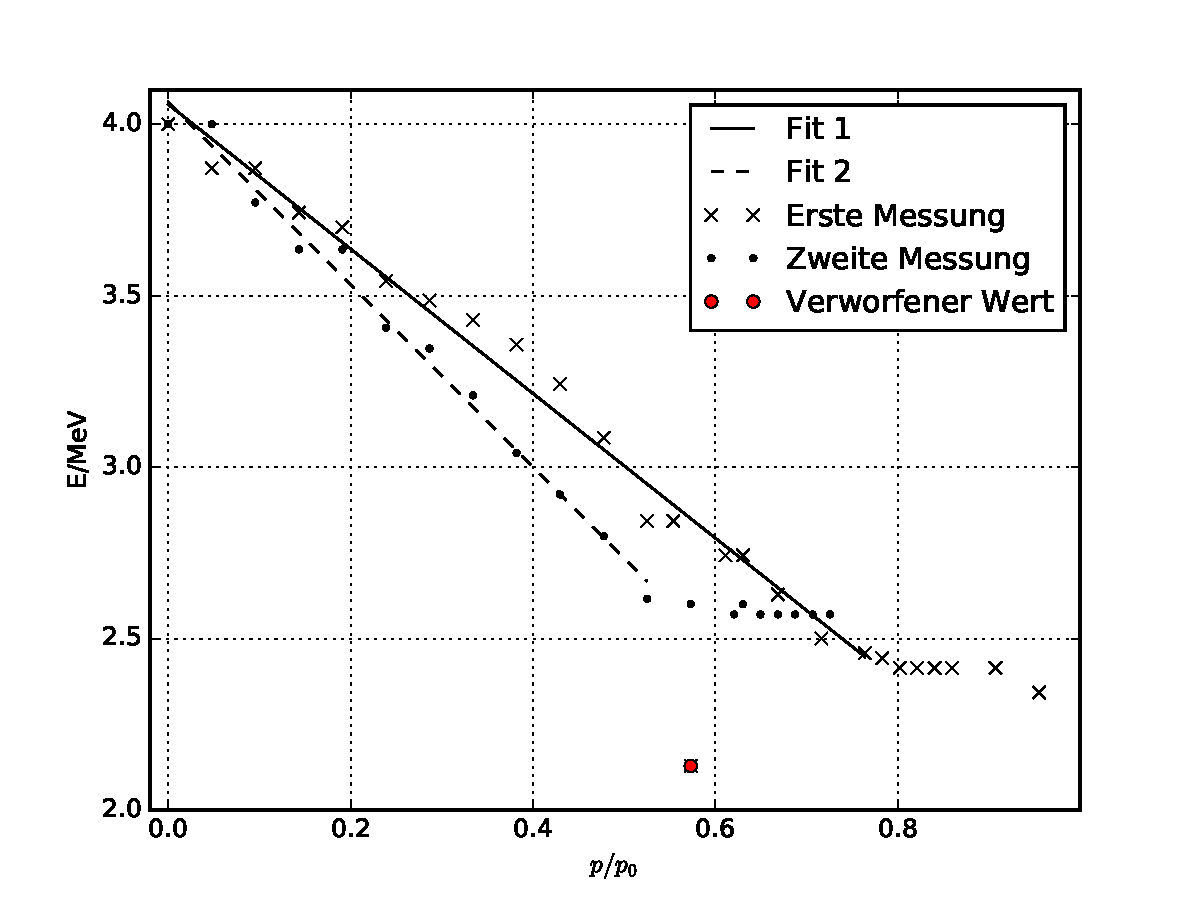
\includegraphics[height=7cm]{plots/Energie.pdf}
  \caption{Energie der gemessenen $\alpha$-Teilchen aufgetragen gegen den relativen Druck $p/p_0$, berechnet aus Tab. \ref{tab:Energie1} und Tab. \ref{tab:Energie2}}
  \label{fig:Energie}
\end{figure}

\begin{table}
  \centering
  \caption{Counts und Kanal maximaler Zählrate zur Bestimmung der druckabhängigen Energie (erste Messreihe).}
  \label{tab:Energie1}
  \begin{tabular}{c c c}
    \toprule
      Druck/mBar & Kanal & Counts \\
      \midrule
      0     & 280 & 70953 \\
      50    & 271 & 71868 \\
      100   & 271 & 72000 \\
      150   & 262 & 70471 \\
      200   & 259 & 70251 \\
      250   & 248 & 69569 \\
      300   & 244 & 68955 \\
      350   & 240 & 68347 \\
      400   & 235 & 67562 \\
      450   & 227 & 66551 \\
      500   & 216 & 63846 \\
      550   & 199 & 56465 \\
      580   & 199 & 59698 \\
      600   & 149 & 59018 \\
      640   & 192 & 56469 \\
      660   & 192 & 57369 \\
      700   & 184 & 56540 \\
      750   & 175 & 52610 \\
      800   & 172 & 47025 \\
      820   & 171 & 45539 \\
      840   & 169 & 21202 \\
      860   & 169 & 16485 \\
      880   & 169 & 13842 \\
      900   & 169 & 18275 \\
      950   & 169 & 2564  \\
      1000  & 164 & 288 \\
      \bottomrule
  \end{tabular}
\end{table}

\begin{table}
  \centering
  \caption{Counts und Kanal maximaler Zählrate zur Bestimmung der druckabhängigen Energie (Zweite Messreihe).}
  \label{tab:Energie2}
  \begin{tabular}{c c c}
    \toprule
      Druck/mBar & Kanal & Counts \\
      \midrule
      0   & 263 & 47993 \\
      50  & 263 & 48432 \\
      100 & 248 & 47334 \\
      150 & 239 & 47048 \\
      200 & 239 & 48851 \\
      250 & 224 & 45413 \\
      300 & 220 & 44444  \\
      350 & 211 & 41207 \\
      400 & 200 & 40080 \\
      450 & 192 & 37177 \\
      500 & 184 & 33282 \\
      550 & 172 & 28074 \\
      600 & 171 & 20380 \\
      650 & 169 & 11543 \\
      660 & 171 & 10012 \\
      680 & 169 & 7151 \\
      700 & 169 & 7151 \\
      720 & 169 & 2494 \\
      740 & 169 & 557 \\
      760 & 169 & 446 \\
      \bottomrule
    \end{tabular}
\end{table}

Für die Plateau-Phase erhält man eine gemittelte Zählrate von $f_1 = \SI{580\pm5}{\becquerel}$, bzw. $f_2 = \SI{377\pm9}{\becquerel}$. Wie Abb. \ref{fig:Rate} zu entnehmen, wurde für den Berreich des stärksten Abfalls ein linearer Fit gemäß \eqref{eqn:gerade} durchgeführt. Die Parameter hierfür sind:
\begin{align*}
  a_{f_1} &= -\SI{4163 \pm 925}{\becquerel} \\
  b_{f_1} &= \SI{3580 \pm 743}{\becquerel} \\
  a_{f_2} &= -\SI{1235 \pm 45}{\becquerel} \\
  b_{f_2} &= \SI{872 \pm 28}{\becquerel}
\end{align*}
Mit diesen Geraden kann man die Mittlere Reichweite der Strahlung durch Umstellung nach dem effektiven Weg und einsetzen von $f_{1/2}$ bzw. $f_{2/2}$ berechnen zu:

\begin{align*}
  R_1 &= \frac{x_o}{a_{f_1}}\left(f_1/2-b_{f_1}\right)=\SI{0.018 \pm 0.006}{\meter} \\
  R_2 &= \SI{0.016 \pm 0.001}{\meter}
\end{align*}

Diese Fehler ergeben sich durch

\begin{align*}
  \Delta R &= \sqrt{\left(\frac{\delta}{\delta a}\frac{x_o}{a_{f}}\left(f/2-b_{f}\right)\right)^2 \cdot \Delta a^2 + \left(\frac{\delta}{\delta b}\frac{x_o}{a_{f}}\left(f/2-b_{f}\right)\right)^2 \cdot \Delta b^2} \\
  &= \sqrt{\left(\frac{x_o}{a_{f}^2}\left(f/2-b_{f}\right)\right)^2 \cdot \Delta a^2 + \left(\frac{x_o}{a_{f}}\right)^2 \cdot \Delta b^2}
\end{align*}


\begin{figure}
  \centering
  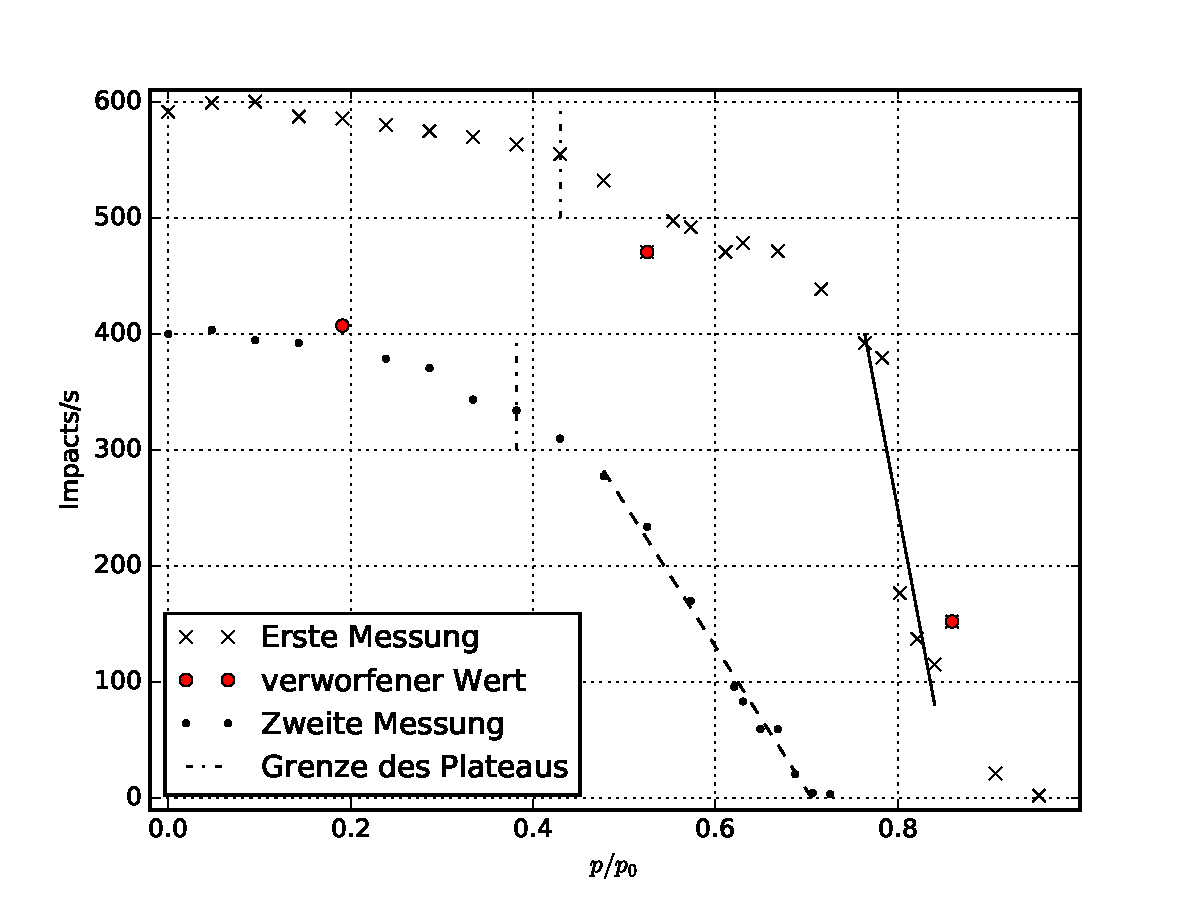
\includegraphics[height=7cm]{plots/Rate.pdf}
  \caption{Zählrate aufgetragen gegen den relativen Druck $p/p_0$}
  \label{fig:Rate}
\end{figure}

\subsection{Statistik des Zerfalls}
Die genommenen Messwerte wurden als normiertes Histogram (d.h. alle Balken addiert ergeben 1) in Abb. \ref{fig:hist} dargestellt, d.h. das Histogram wurde so normiert, dass die Summe über alle Balken 1 beträgt. Die eingezeichnete Fit-Kurve stellt eine Gauß-Normalverteilung gemäß
\begin{equation}
  G(x) = \frac{A}{\sigma\cdot\sqrt(2\pi)}e^{-0.5 \left(\frac{x-m}{\sigma}\right)^2}
  \label{eqn:gauß}
\end{equation}
dar. Hierbei ist  $\sigma=\SI{19.81 \pm 1.07}{\becquerel}$ die Standardabweichung und $m= \SI{533.98}{\becquerel}$ der Mittelwert der aufgenommenen Werte. Im Histogram sind 10 Balken aufgelöst, was einer Breite von ca. $\SI{10}{\becquerel}$ entspricht und somit höher auflösend gewählt ist als die Standardabweichung.

 \begin{figure}
   \centering
   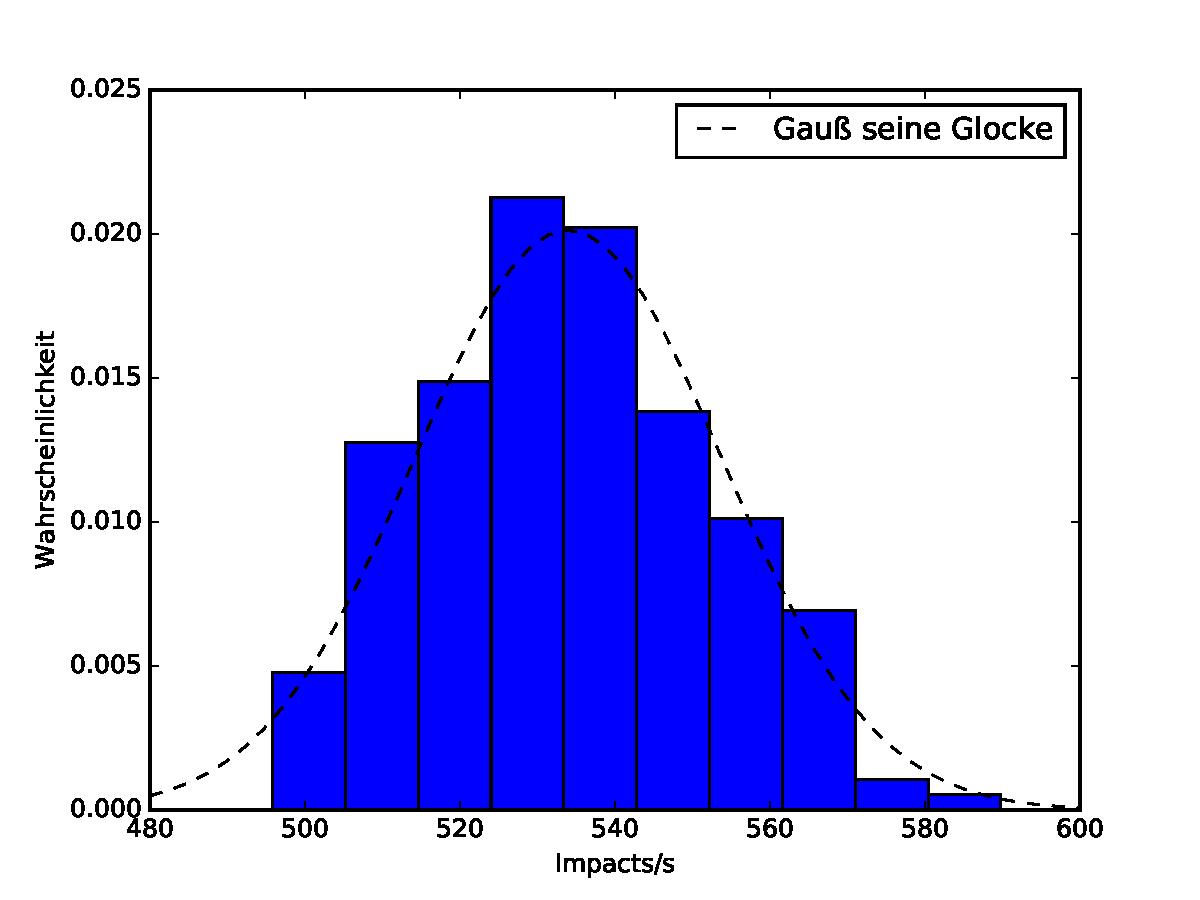
\includegraphics[height=7cm]{plots/Statistik.pdf}
   \caption{Histogram zur Zählrate mit Gauß-Verteilung}
   \label{fig:hist}
 \end{figure}

Der Poisson-Fit ist in Abb. \ref{fig:fisch} dargestellt und liefert den Parameter
\begin{equation*}
  \lambda = 6.8 \pm 0.3
\end{equation*}
Die Poisson-Verteilung ist gegeben durch
\begin{equation*}
  P(k) = \frac{\lambda^k}{k!}e^{-\lambda}.
\end{equation*}
Rechnet man dies in den tatsächlichen Erwartungswert $\lambda_{real} = 5 \cdot(\lambda +100)$, so ergibt sich $\lambda_{real} = \SI{534.0 \pm 1.5}{\becquerel}$.
\begin{figure}
  \centering
  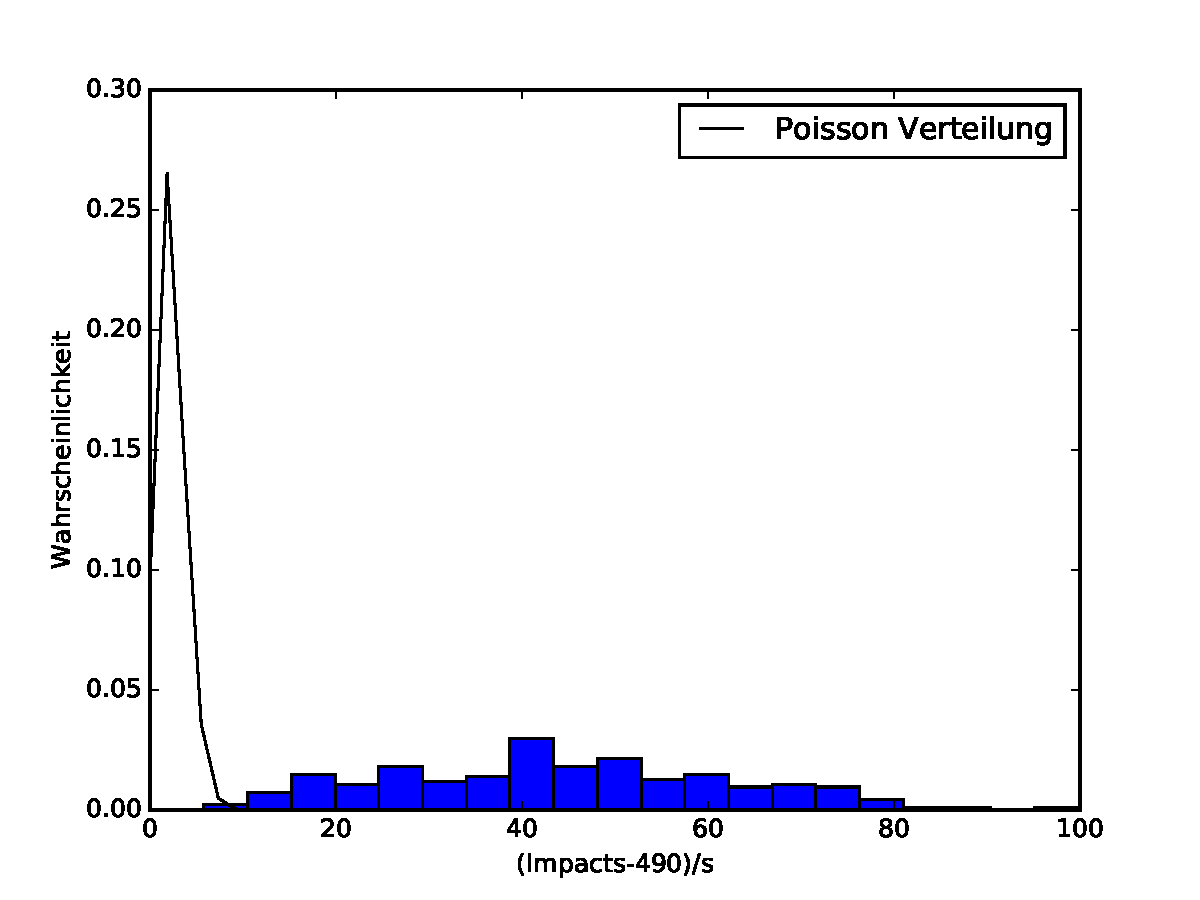
\includegraphics[height=7cm]{./plots/Poisson.pdf}
  \caption{Histogram zur Zählrate mit Poisson-Verteilung.}
  \label{fig:fisch}
\end{figure}
